\documentclass[12pt]{article}
\title{Report of "Autocorrelation In Weather"}
\author{Hongye Wang}
\date{December 2019}
\usepackage{graphicx}
\usepackage{float}

\DeclareUnicodeCharacter{2212}{-}

\begin{document}
  \maketitle

  \section{Introduction}
    Autocorrelation in weather: The goal is to answer the question: Are temperatures of one year significantly correlated with the next year (successive years), across years in a given location? For this, I calculated the correlation between n−1 pairs of years, where n is the total number of years. However, the standard p-value can not be used for a correlation coefficient, because measurements of climatic variables in successive years are in a time series but not independent. 

  \section{Methods}
    1.Compute the appropriate correlation coefficient between successive years
    2.Repeat this calculation 10000 times by -- randomly permuting the time series, and then recalculating the correlation coefficient for each randomly permuted year sequence
    3.Then calculate what fraction of the correlation coefficients from the previous step were greater than that from step 1 (this is the approximate p-value)

  \section{results}
    Pvalue is not a constant value because the samples are random. P value = n*e-04(n is not constant but less than 10). As I set seed in R code, the P value is constant at e-04.
    
    \begin{figure}
      \centering
      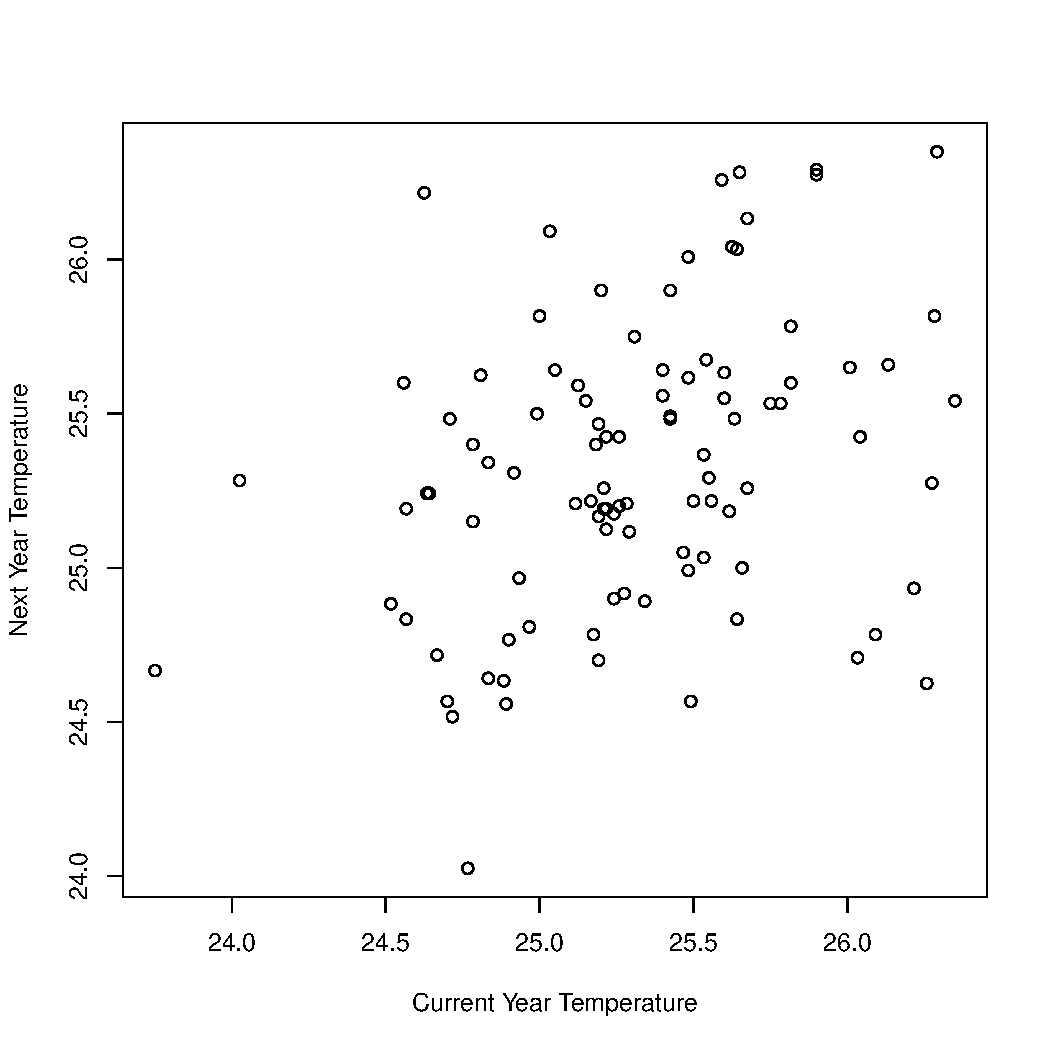
\includegraphics[width = \textwidth]{../result/TAutoCorr_plot1.pdf}
      \caption{This is a pattern shows the correlation between current year temperature and next year's}
    \end{figure}
    
    \begin{figure}
      \centering
      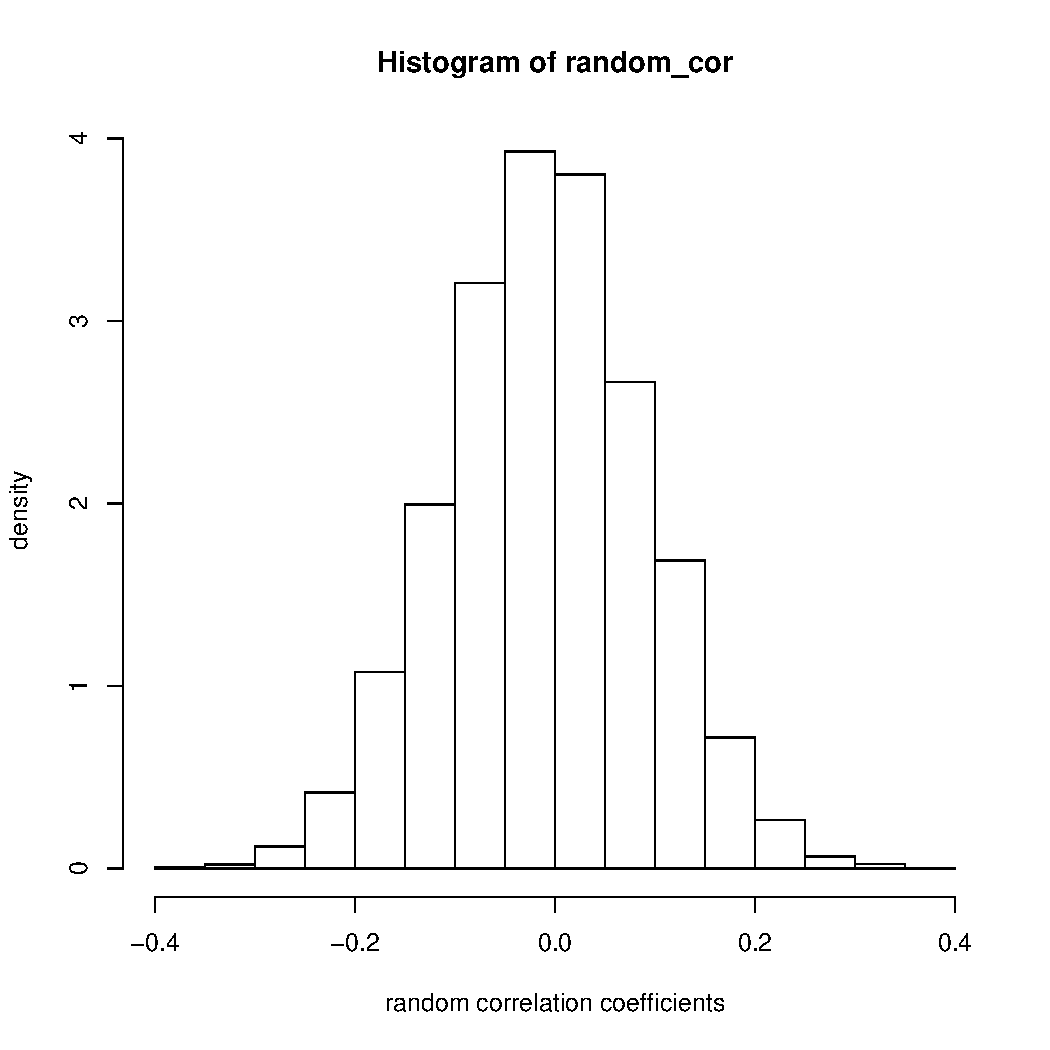
\includegraphics[width = \textwidth]{../result/TAutoCorr_plot2.pdf}
      \caption{The histogram presents the permuted correlation coefficients frequence.}
    \end{figure}

  \section{interpretation}
    P value is pretty small (0.0001), which shows confidently that there is a positive correlation between current year mean temperature and its next year's temperature. The 10000 times experiments of calculating the permuted annual mean temperatures present that the correlation between successive year's temperatures is bigger than most other correlations between randomly two years.

\end{document}
\grid